% 3. Anatomical Models
\section{Anatomical Models}
% - quello di agnello (al-jumaily2011)
% - un altro (herrmann2016)

% I modelli matematici sviluppati per i polmoni degli adulti non possono
% essere semplicemente ridotti in scala per adattarsi ai polmoni dei
% neonati. Infatti, i polmoni dei neonati non sono semplicemente una
% versione in miniatura dei polmoni degli adulti, ma presentano
% differenze significative in termini di proporzioni dei rami
% bronchiali, costituenti delle vie aeree, caratteristiche morfometriche
% e composizione. Queste differenze devono essere prese in
% considerazione quando si sviluppano o si adattano modelli matematici
% per rappresentare accuratamente il funzionamento dei polmoni dei
% neonati. La struttura dei polmoni dei neonati presenta proporzioni
% diverse rispetto a quella degli adulti. Le diramazioni delle vie aeree
% possono avere dimensioni e disposizioni differenti.  I componenti dei
% polmoni, come il tessuto e le cellule, possono variare tra neonati e
% adulti.  Gli studi morfometrici, che analizzano la forma e la
% struttura dei polmoni, mostrano che ci sono differenze tra neonati e
% adulti che devono essere considerate nei modelli.  Ci sono differenze
% nella composizione del tessuto polmonare tra neonati e adulti che
% influenzano come i polmoni funzionano e rispondono alle terapie.

% The hierarchy of the dividing airways largely determines the internal
% lung structure, which is a fractal branching tree\cite{suki2011}. The
% structural design of the airway tree is functionally important because
% the branching pattern plays a role in determining air flow and
% particle deposition. In modeling the human airway tree, it is
% generally agreed that the airways branch according to the rules of
% irregular dichotomy.  Regular dichotomy means that each branch of a
% treelike structure gives rise to two daughter branches of identical
% dimensions. In irregular dichotomy, however, the daughter branches may
% differ greatly in length and diameter.

The structure of the internal lung is significantly influenced by the
hierarchical arrangement of the airways, which resemble a fractal
branching tree\cite{suki2011}. The design of this airway tree is
crucial for its function, as the branching pattern affects both
airflow and particle deposition. In modeling the human airway tree, it
is widely accepted that the airways follow an irregular dichotomy
pattern. Unlike regular dichotomy, where each branch splits into two
identical daughter branches, irregular dichotomy results in daughter
branches that can vary significantly in length and diameter.

\begin{figure}[H]\centering
  % 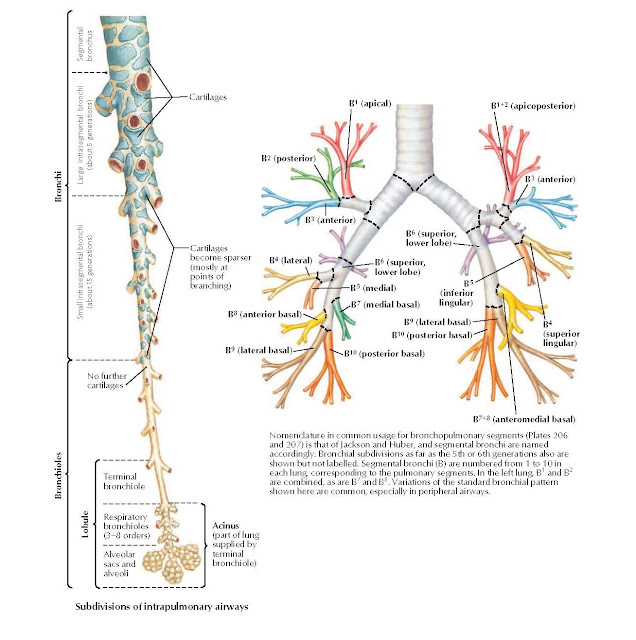
\includegraphics[width=\textwidth]{airway_tree_best.jpg}
  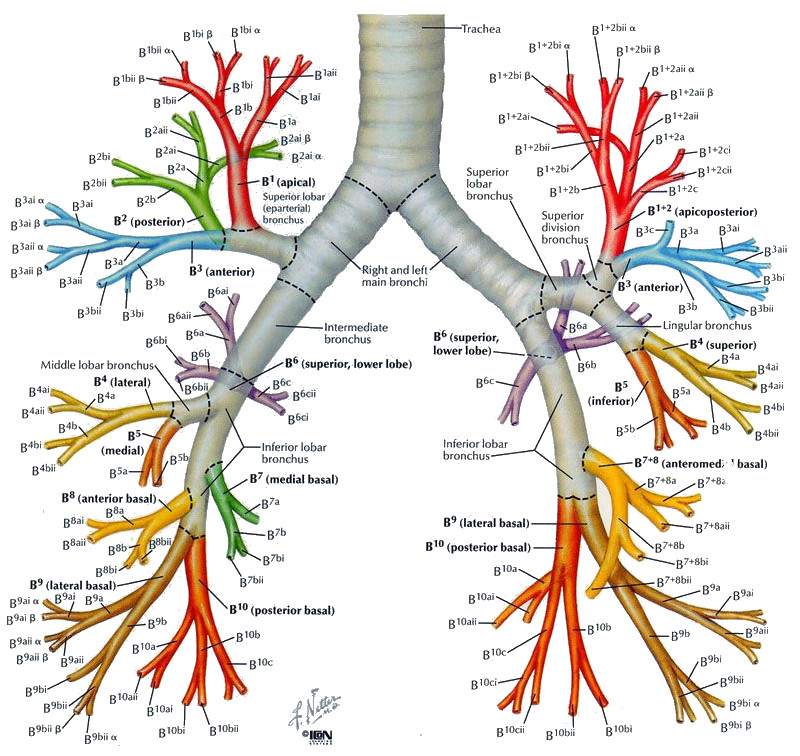
\includegraphics[width=.8\textwidth]{airway_tree_no_left_best.jpg}
  \caption{Representation of the major airways.}
  \label{fig:airway_tree_anatomical}
\end{figure}

Mathematical models developed for adult lungs cannot simply be scaled
down to fit the lungs of newborns. In fact, newborn lungs are not
simply one miniature version of adult lungs, but they present
significant differences in terms of bronchial branch proportions,
constituents of the airways\cite{merkus1996}, morphometric
characteristics\cite{horsfield1987} and
composition\cite{hislop1989}. These differences must be taken into
account when developing or adapting mathematical models to accurately
represent the functioning of the lungs of the newborns. The structure
of the lungs of newborns presents proportions different than that of
adults. The branches of the airways they can have different sizes and
arrangements. The components of lungs, like tissue and cells, can vary
between newborns and adults. Morphometric studies, which analyze the
shape and the structure of the lungs, show that there are differences
between newborns and adults that need to be considered in the
models\cite[][Ch. 1.1]{mani2020}. There are differences in the
composition of lung tissue between newborns and adults who influence
how the lungs function and respond to therapies.

%% Citare qui i riferimenti che ha fatto chiara nella call del 21.06

\textcite{mani2020} considered an adult lung model linearly scaled to
match newborn anatomical features.  The advantage of this approach is
that it respects the dimensions of trachea and bronchioles. It doesn't
guarantee that the morphometric characteristics of the entire airway
tree are respected.  In this work, there are few airway generation
parameters that can in fact be adapted, in order to better approximate
the target morphometric characteristics.

% Modello ovino (al-jumaily2011) e di Jacob (herrmann2016).

% GESTISCI IMMAGINE E TESTO SOTTO
\begin{figure}[H]\centering
  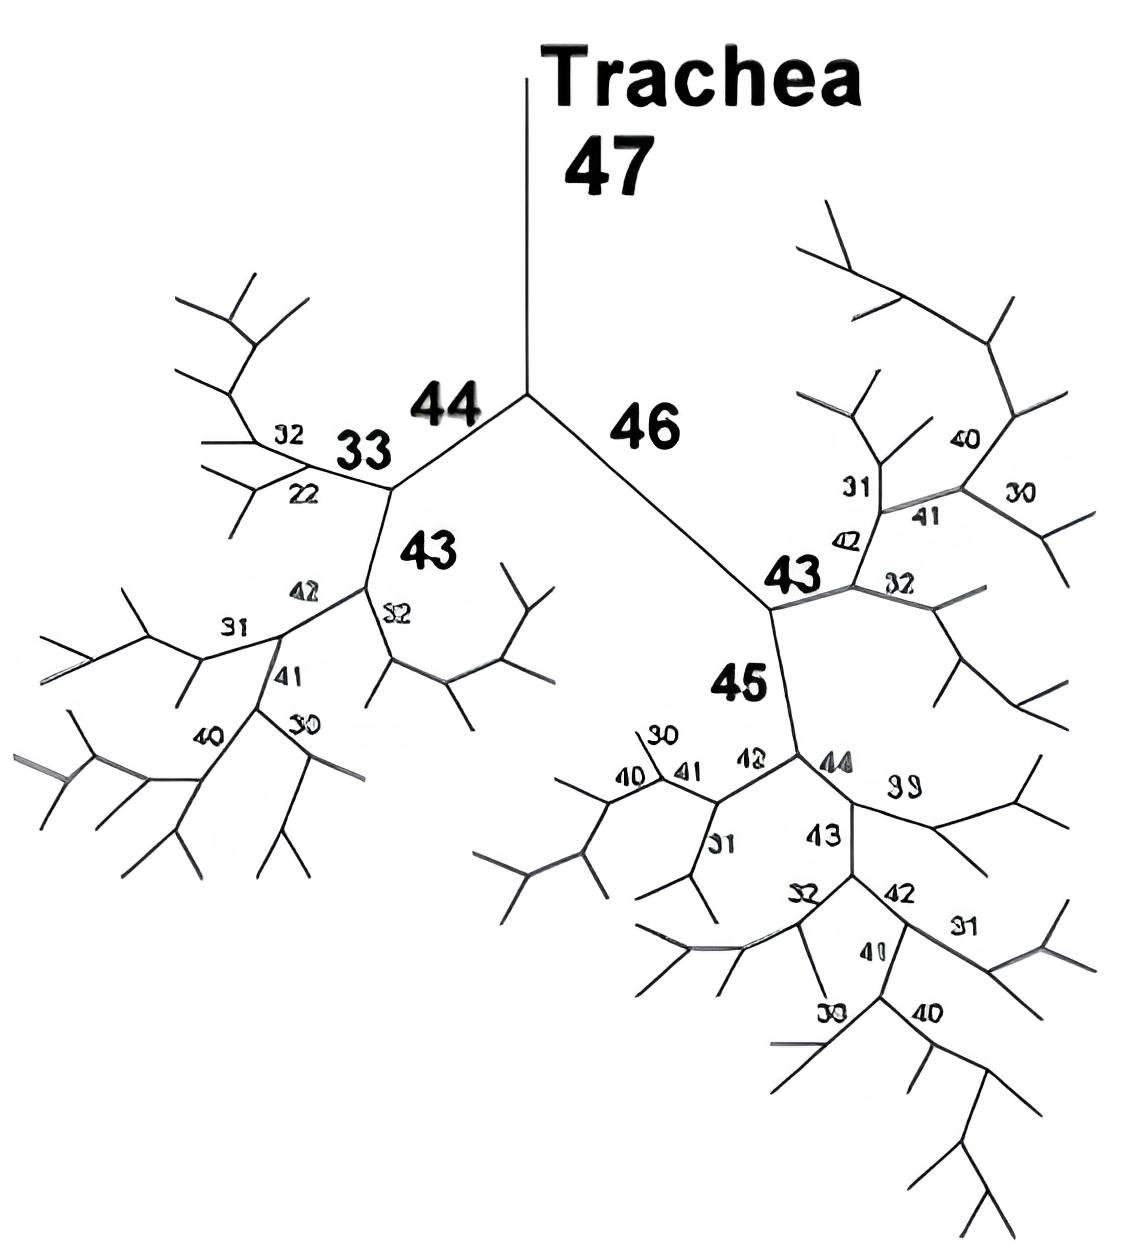
\includegraphics[width=.5\textwidth]{albero_dicotomico_best.png}
  \caption{The dichotomous bronchial tree.}
  \label{fig:albero_dicotomico_anatomical}
\end{figure}

% Prendo quest'immagine e spiego che l'albero che sto considerando può
% essere modellizzato come un albero dicotomico, cioè che si divide
% sempre in due ed in cui sono sempre diversi gli angoli, le lunghezze,
% possono avere diramazioni diverse e quindi proprietà diverse.

% AGGIUNTA QUESTA MODIFICA, COMPLETARE
% -> spiegato il concetto in inglese.
\Cref{fig:albero_dicotomico_anatomical} serves as a reference for
constructing anatomically coherent adult lungs. In a dichotomous tree,
each airway (excluding the trachea) has a single parent branch and two
daughter branches (excluding the acini).  Asymmetrical bronchial trees
are a specific class presenting uneven splitting: Horsfield orders of
two siblings are in fact different (causing recursion index $\Delta$
to exist, see \cref{fig:airway_impedance}).  Branching angles, lengths
and diameters can vary, resulting then in different mechanical
properties.

Newborn lung can be considered as having an analogous structure.

% LEGGERE INTRONORA E TAWHAI, POI CAPIRE COME CITARLI IN QUESTO PUNTO.
Da tac, .. estratto centerline e ricostruito con diversi algoritmi la parte
mancante (Nora, Tawn..).

% Questa struttura in \Cref{fig:albero_dicotomico_anatomical} è stata
% usata come riferimento per la costruzione di alberi brochiali
% anatomicamanete coerenti per applicazioni su adulti. 

% PER CITARE NORA: \cite{tgavalekos2003}, PER CITARE TAWHAI
% \cite{tawhai2000}

Instead for infants, there exist models based on the
ovine\cite{al-jumaily2011} and canine\cite{herrmann2016} anatomy.

%%% Local Variables:
%%% mode: LaTeX
%%% TeX-master: "../Thesis"
%%% End:
